\subsection{Zielsetzung}

Ziel dieser Arbeit ist die Entwicklung eines WebApp-Wrappers, eine Vorlage, mit der Webentwickler eine Webseite mit geringem Aufwand in eine Anwendung verpacken können, die für alle gängigen Desktop- und Mobile"=Plattformen (Windows, Linux, macOS, Android und iOS) kompiliert werden kann.

Um den Funktionsumfang der Anwendung zu erweitern, soll es möglich sein, ein Node.js Projekt zu integrieren.

Der WebApp-Wrapper soll eine vorgefertigte Benutzeroberfläche mitliefern, welche einen Ladebildschirm, einen Fehlerbildschirm, ein Meldungsfenster und eine Menüleiste umfassen soll.

Darüber hinaus soll eine einfache \ac{api} zur Verfügung gestellt werden, um die Anpassung der Anwendung an die individuellen Bedürfnisse zu ermöglichen.

Weitere Einzelheiten über die Funktionalitäten sind im Kapitel \hyperref[sec:WebApp-Wrapper]{WebApp-Wrapper} zu finden.

\begin{figure}[H]
    \centering
    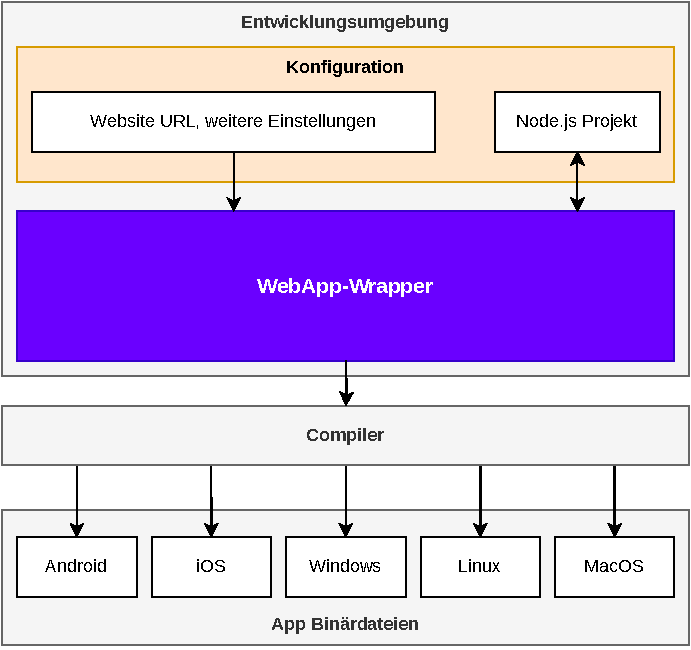
\includegraphics[width=0.8\textwidth]{assets/01_Einführung/02_Zielsetzung.drawio.pdf}
    \caption[Zielsetzung]{Zielsetzung}
\end{figure}
